\documentclass{article}
\usepackage{xcolor}
\usepackage[a4paper, top=0.5in, bottom=0.5in, left=0.6in, right=0.6in]{geometry}

\pagecolor[rgb]{0.06,0.06,0.06}
\color[rgb]{1,1,1}
% Language setting
% Replace `english' with e.g. `spanish' to change the document language
\usepackage[english]{babel}
% Set page size and margins
% Replace `letterpaper' with `a4paper' for UK/EU standard size
\usepackage[letterpaper,top=2cm,bottom=2cm,left=3cm,right=3cm,marginparwidth=1.75cm]{geometry}

% Useful packages
\usepackage{amsmath}
\usepackage{graphicx}
\usepackage[colorlinks=true, allcolors=yellow]{hyperref}
\renewenvironment{abstract}{
    \begin{center}
        \textbf{Description} % Custom title centered and bold
    \end{center}
    \noindent
}{
    \par\vspace{0em}
}
\title{\textbf{Encrypted Ballot}}
\author{Rachit Kumar Pandey \\ IIT (ISM) Dhanbad}
\date{}

\begin{document}
\maketitle

\begin{abstract}
The project aims to develop a secure voting system that ensures voters can cast their votes both anonymously and without the possibility of being traced back. It also uses partial trustees to ensure there is no single point of failure.
\end{abstract}
\section*{\centering Stakeholders}
\begin{center}
    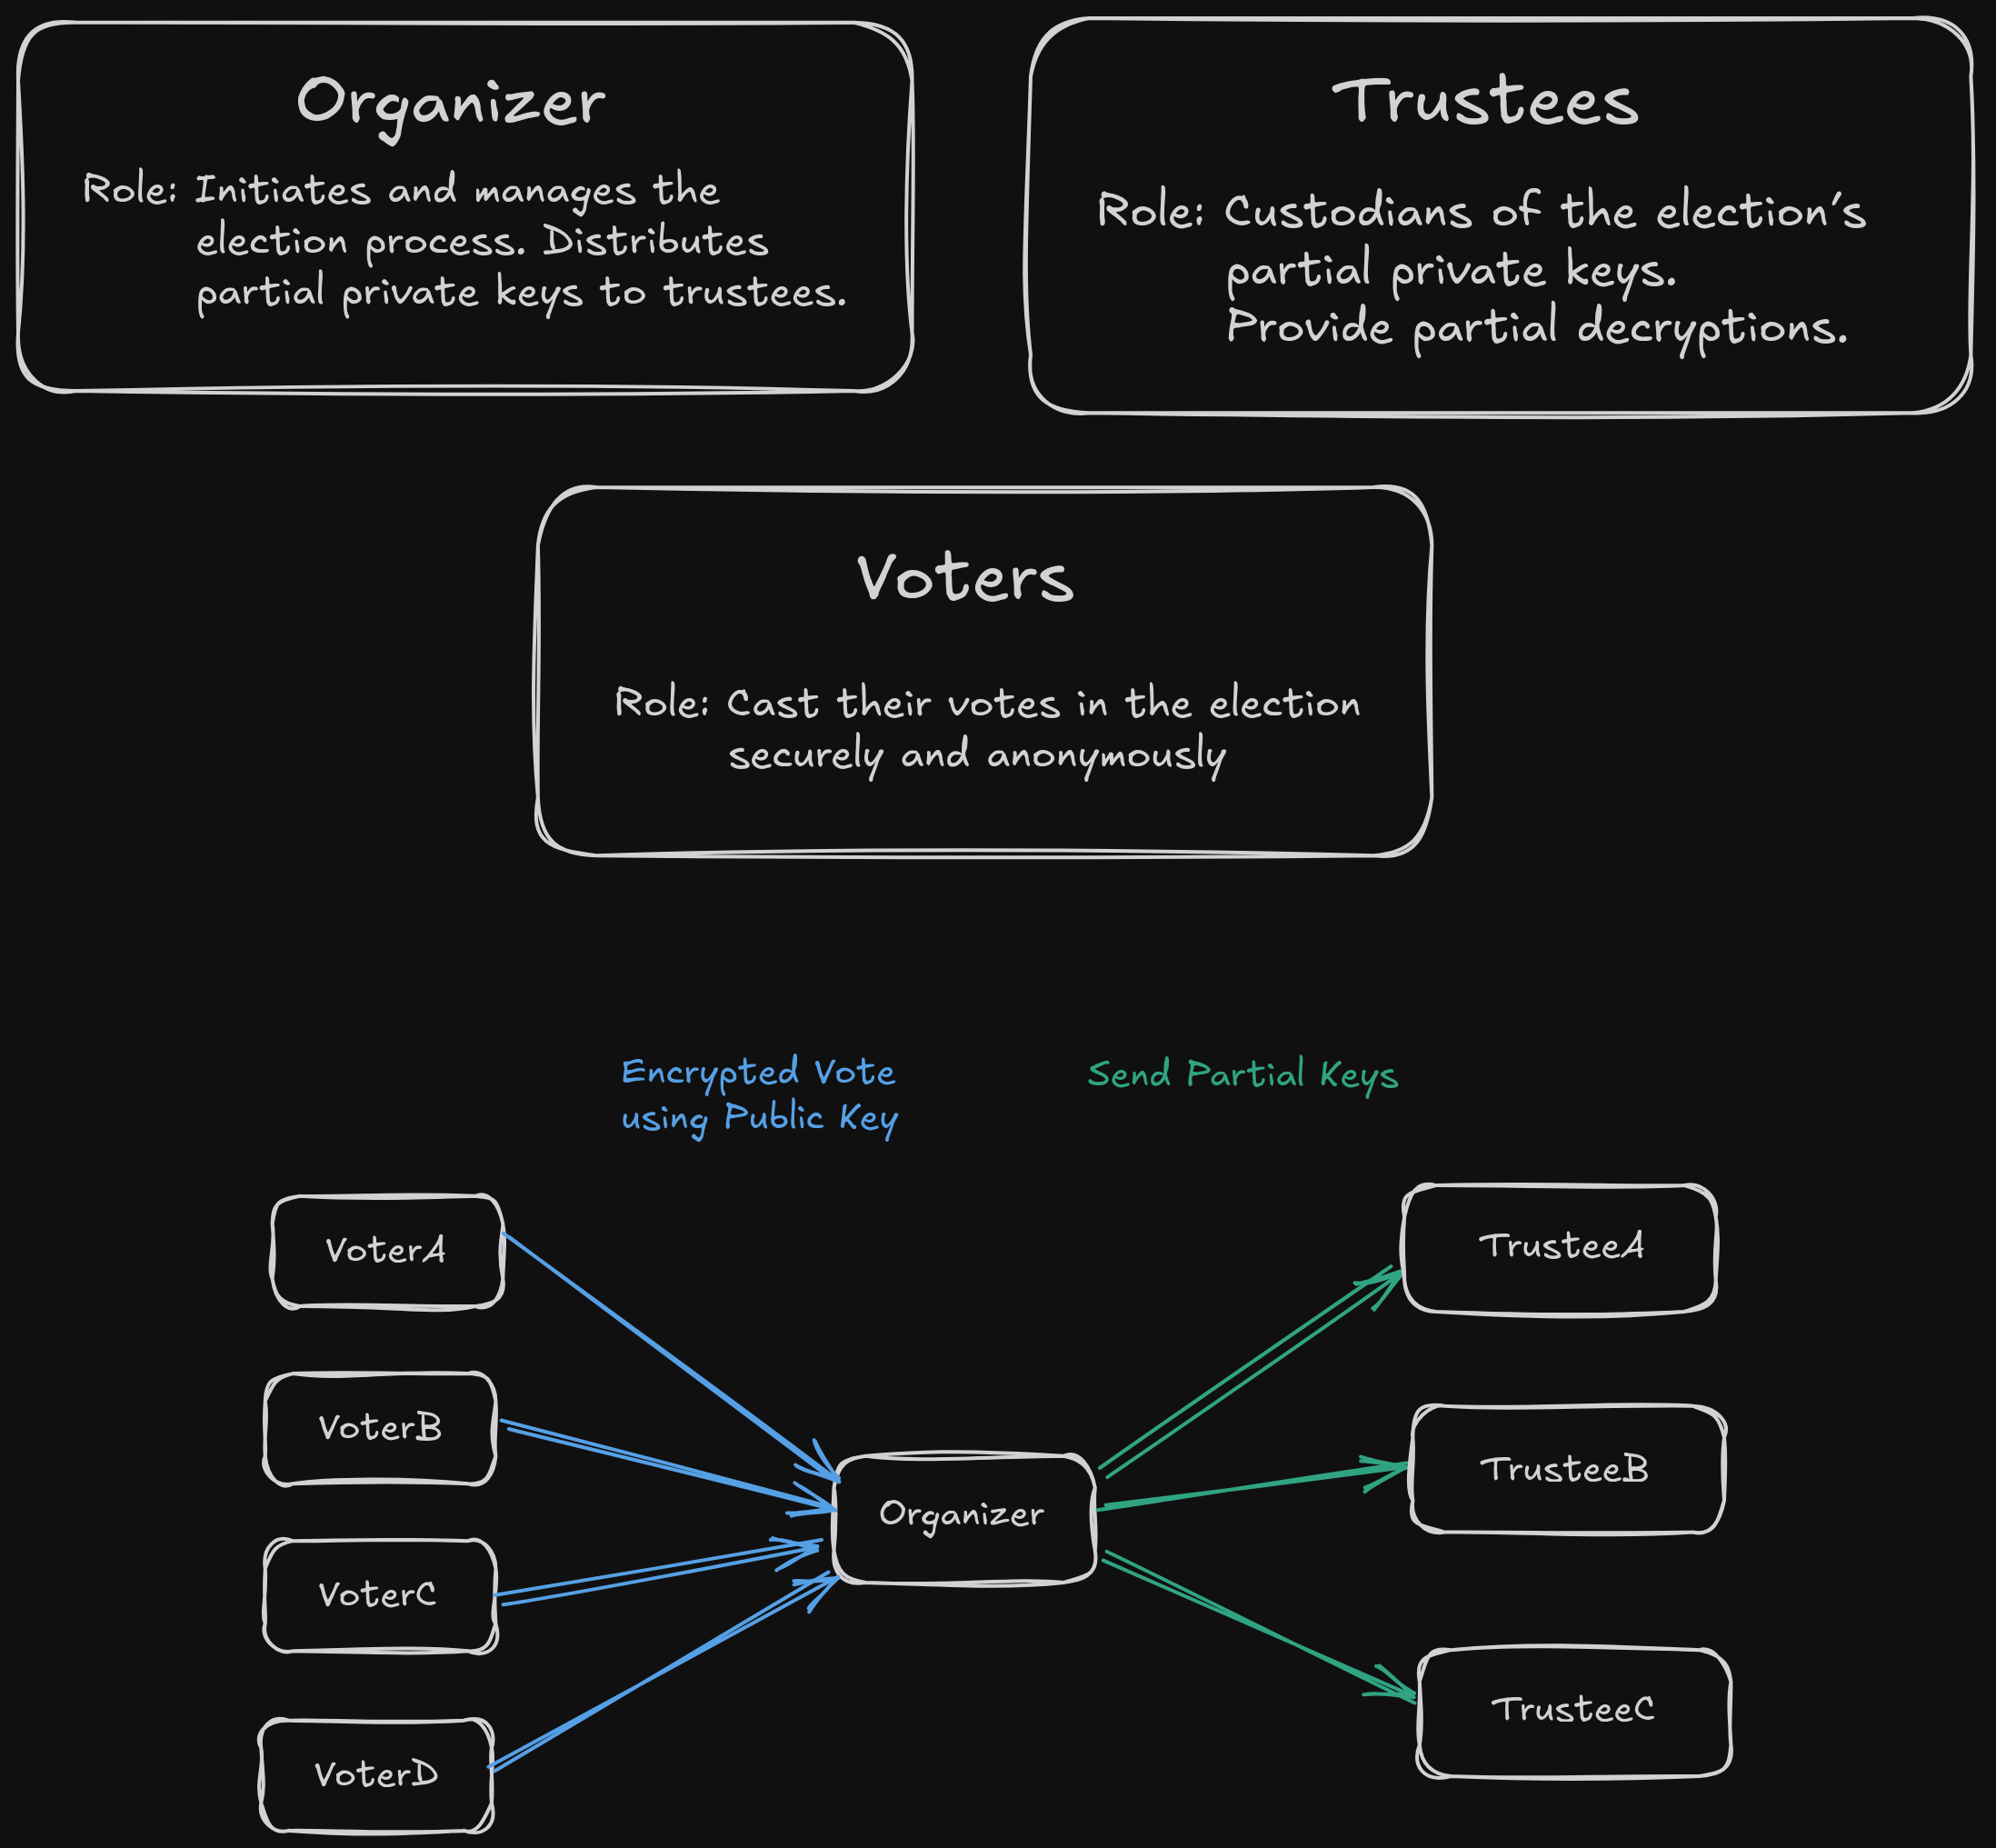
\includegraphics[width=\textwidth]{stakeholders.png}
\end{center}
\begin{centering}
    
\end{centering}
\pagebreak
\begin{center}
    \section*{The Plan}
    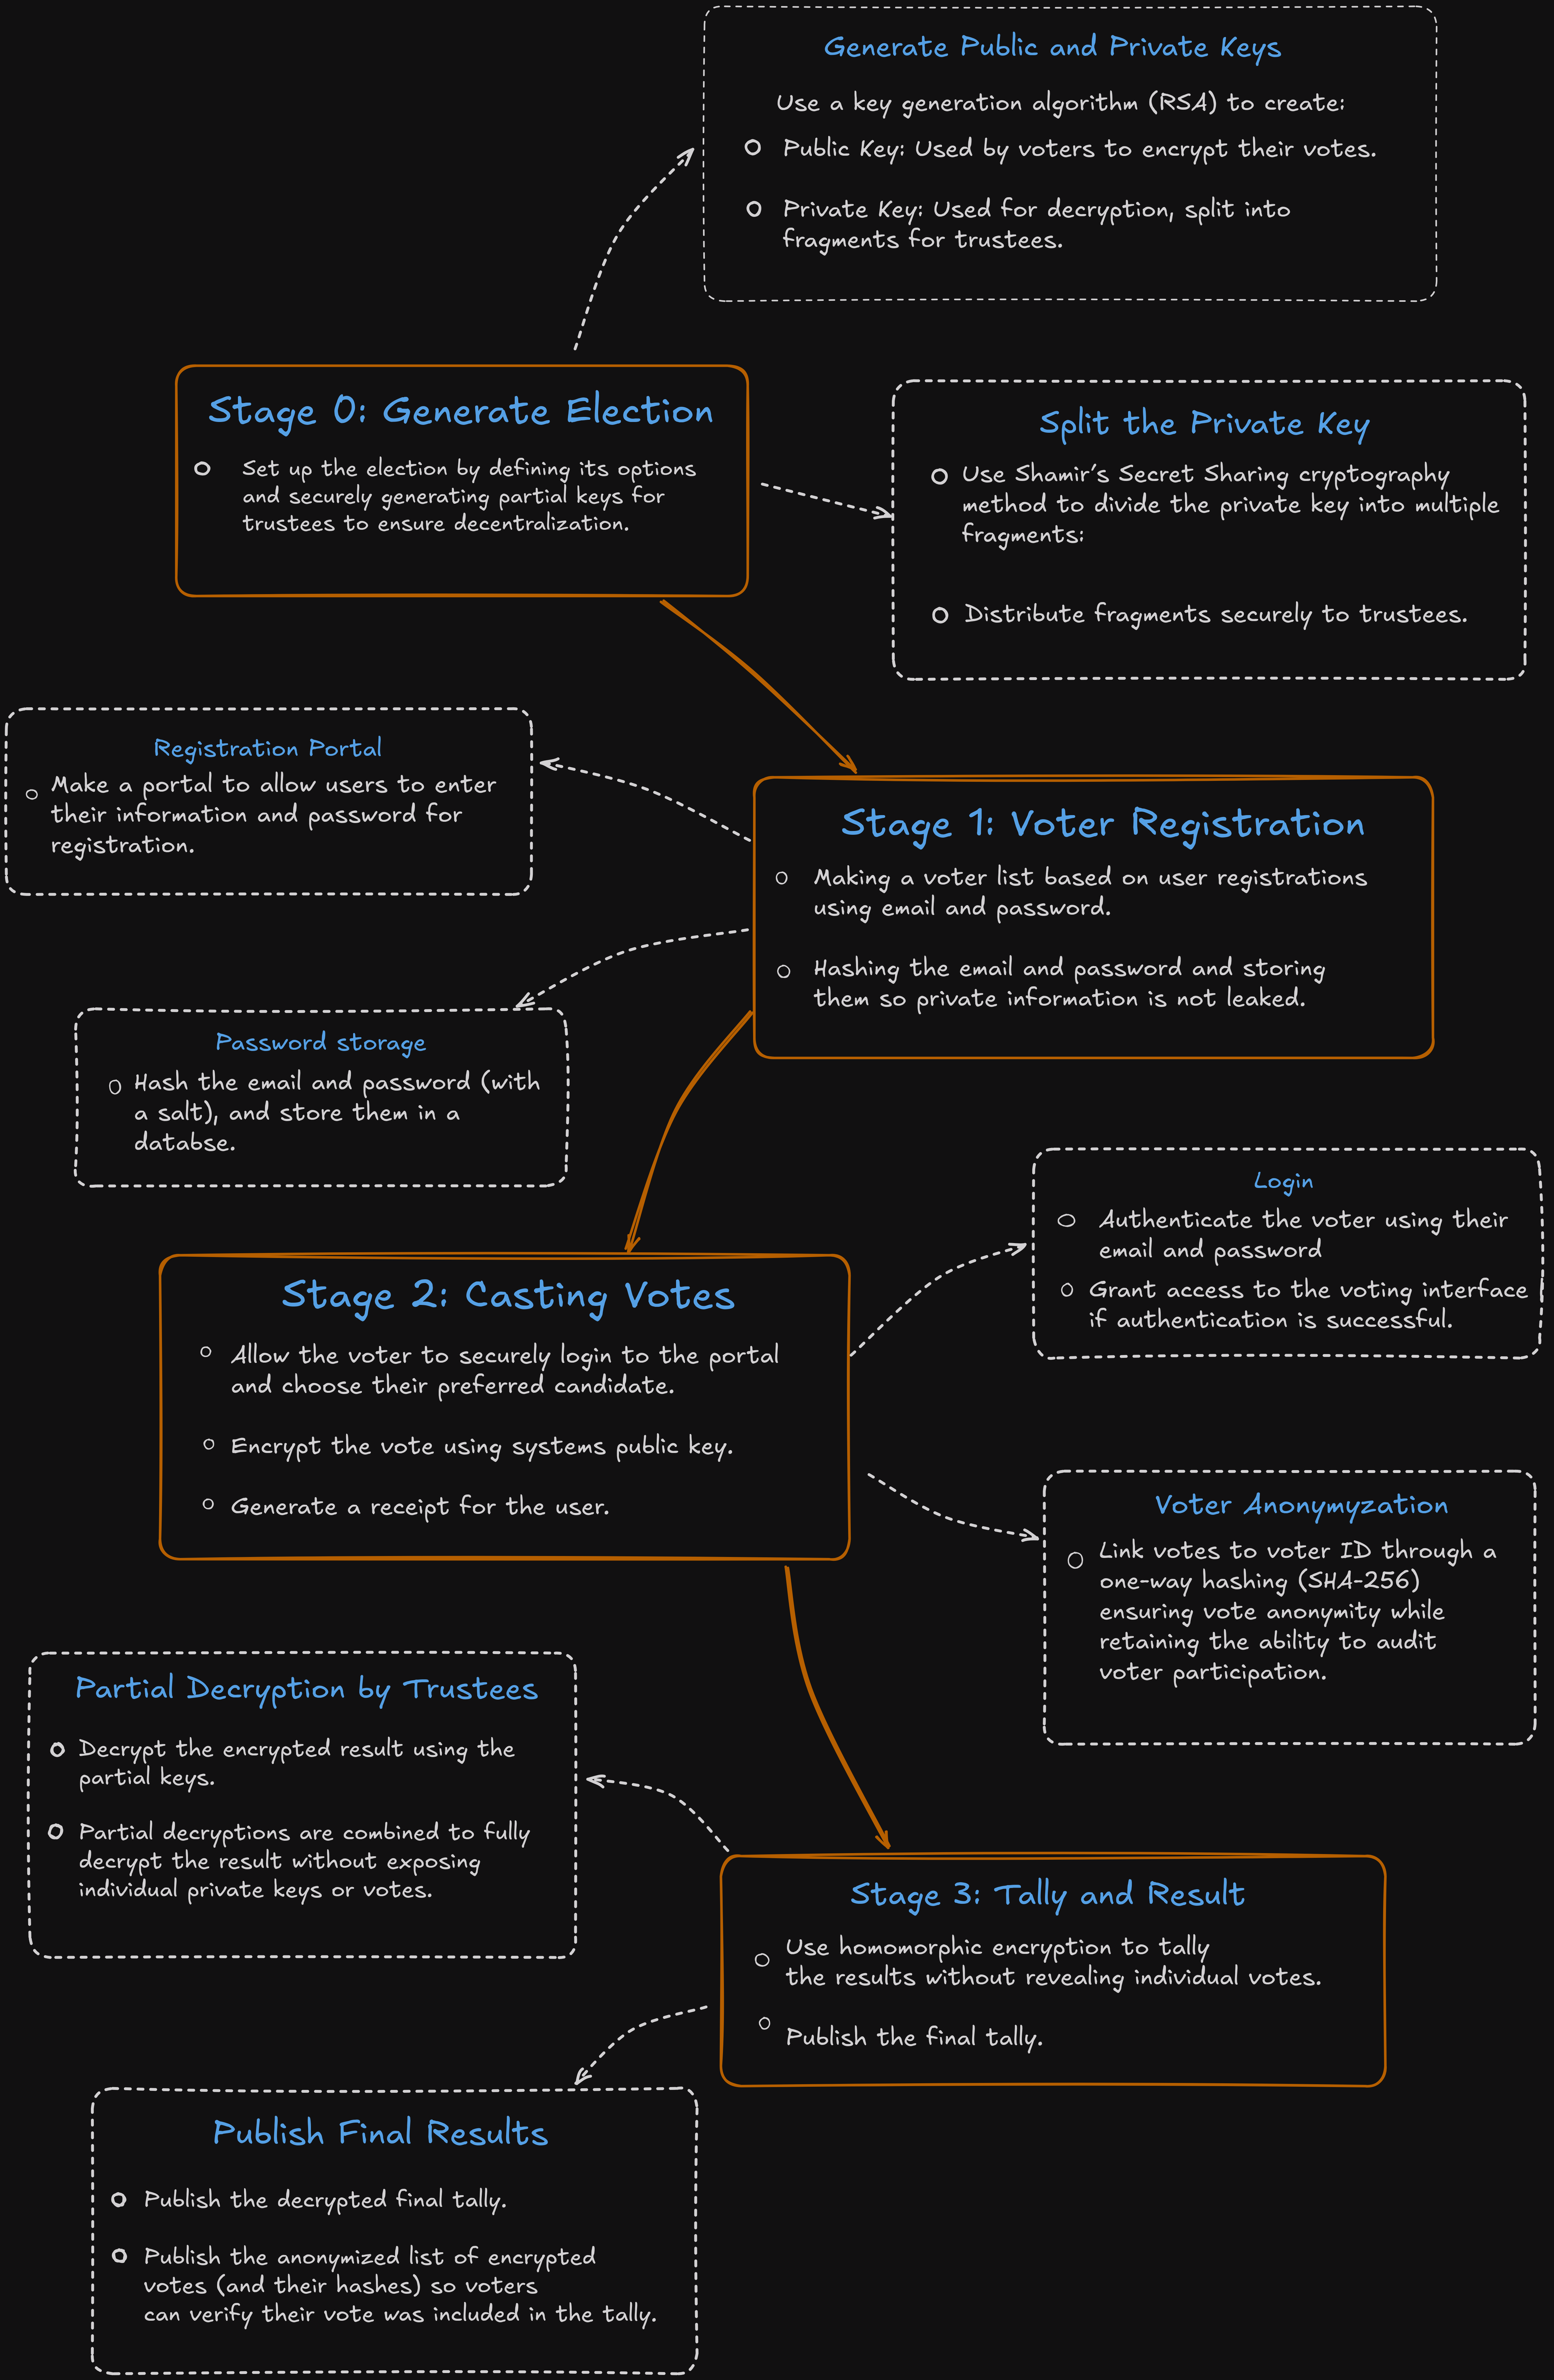
\includegraphics[width=\textwidth]{plan.png}
\end{center}

\pagebreak
\section*{\centering Tech Stack}

\includegraphics[width=\textwidth]{techstack.png}

\section*{\centering Timeline}
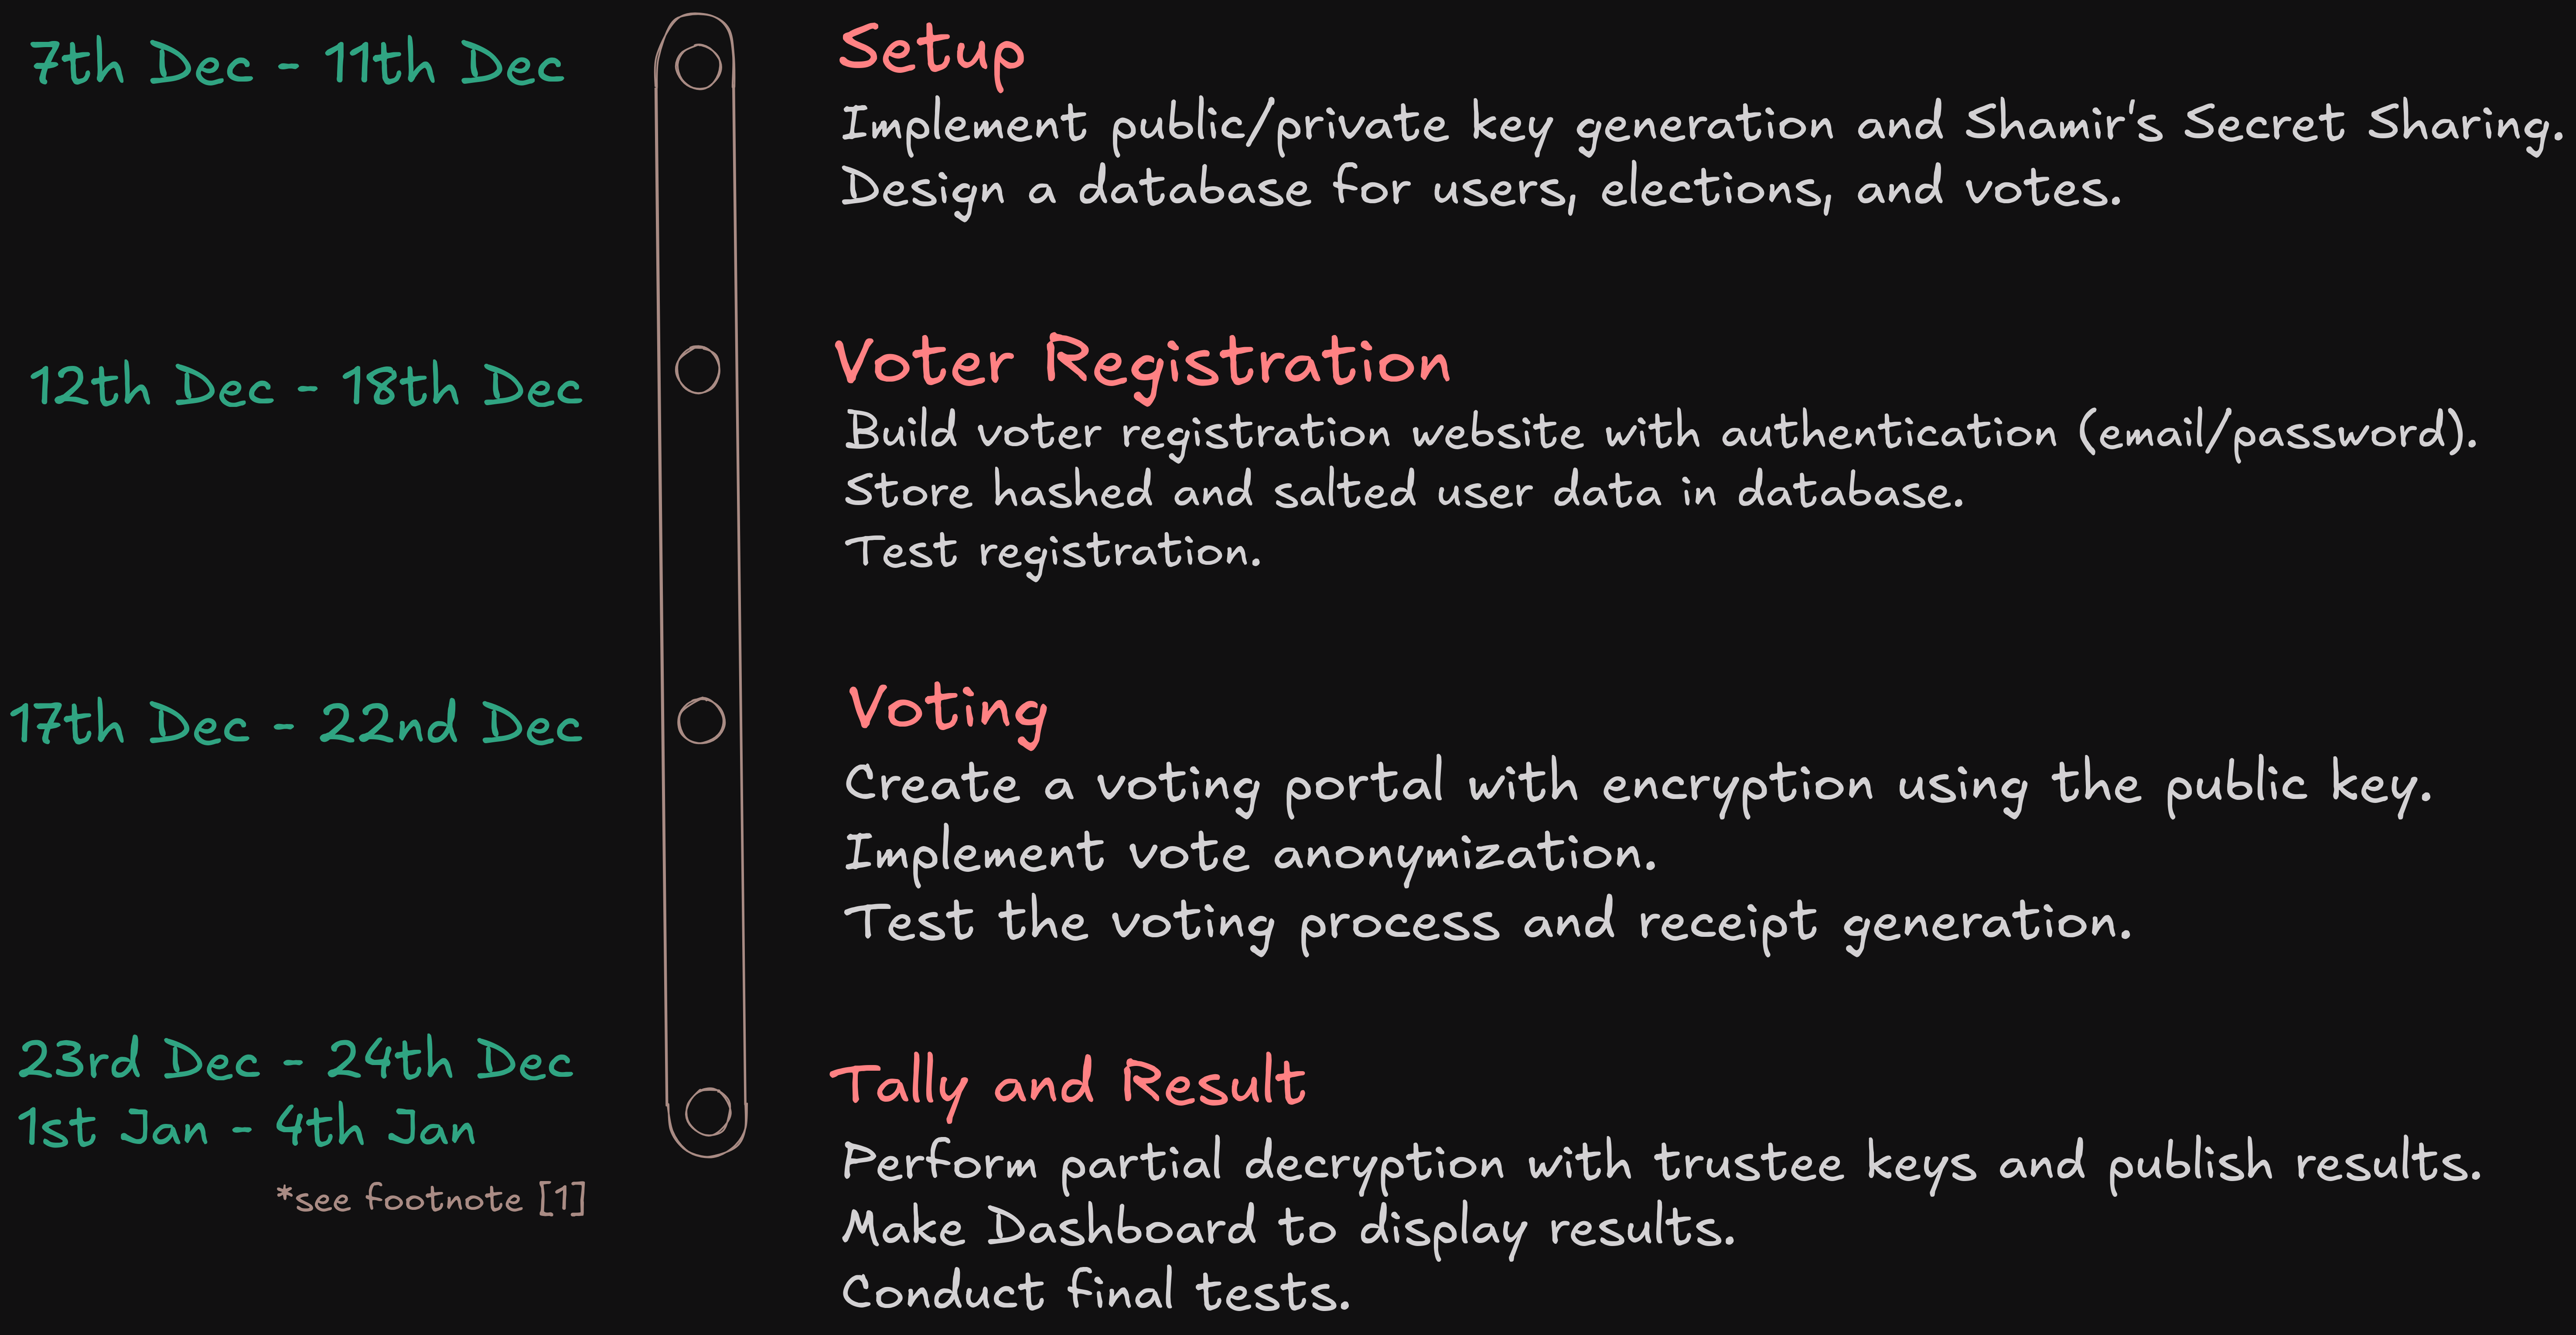
\includegraphics[width=\textwidth]{timeline.png}
\\
\\
\section*{\centering About Me}
\begin{itemize}
\setlength{\itemsep}{1pt} % Adjust spacing between items
  \setlength{\parskip}{0pt}
  \renewcommand{\labelitemi}{\hspace*{-1em}} % Remove the bullet
   \item Just a guy curious about tech.
   \\
\item My dive into this world began when I was around 15 years old. I wanted to understand how computers work, which led me to start learning basic digital electronics.
\\
\item As I explored further, I discovered a completely different operating system that was said to be much closer to the hardware. Intrigued, I decided to wipe my hard drive clean and install Linux and fell down the rabbithole. I haven’t gone back to Windows ever since.
\\
\item I also had some experience with cryptography while learning about email encryption and hash verification. However, I never explored it much further, which is exactly why I chose this project.
\end{itemize}
\section*{\centering Why Me?}
\begin{itemize}
\setlength{\itemsep}{1pt} % Adjust spacing between items
  \setlength{\parskip}{0pt}
  \renewcommand{\labelitemi}{\hspace*{-1em}} % Remove the bullet
   \item I truly love this field and I'm really passionate about it.\\
    I’m confident I can learn, grow, and contribute in the club effectively in the club.\\
\end{itemize}
Due to my impulsive nature, I can't commit any daily goal but I will commit about 30-35 hours per week.
I'll also try to maintain and keep updated a Github repository linked \href[color=yellow]{https://github.com/armoredvortex/woc}{\underline{here.}}
\setcounter{footnote}{1}
\footnotetext{I'll be going on a trip from 25th-31st Dec, I'll be taking my laptop along but I don't believe I'll be able to get any significant work done. Hence I've excluded that period from the timeline.}

\end{document}